% Generated from reviewed lane; compile via book/textbook.tex.
\clearpage

原书 PDF 页 1；无印刷页码。

\href{source-images/pdf-001.jpeg}{查看原页}

普通高等教育``十三五''规划教材\\
普通高等院校数学精品教材

十三五

获教育部高等学校优秀教材二等奖\\
获全国优秀畅销书奖

\section{数值分析}\label{front-ux6570ux503cux5206ux6790}

第 5 版

李庆扬　王能超　易大义　编

\begin{itemize}
\tightlist
\item
  强调基本原理、基本理论，夯实基本素质
\item
  注重基本方法和技巧，提高应用能力
\item
  阐述严谨，脉络分明，深入浅出
\item
  反复锤炼，不断更新，长销 30 余年
\end{itemize}

华中科技大学出版社\\
\url{http://www.hustp.com}

\begin{quote}
版式记录（agent 补充）：本页为封面，无印刷页码。``十三五''也出现在封面徽标及背景装饰中；完整图形与字样见原页。
\end{quote}

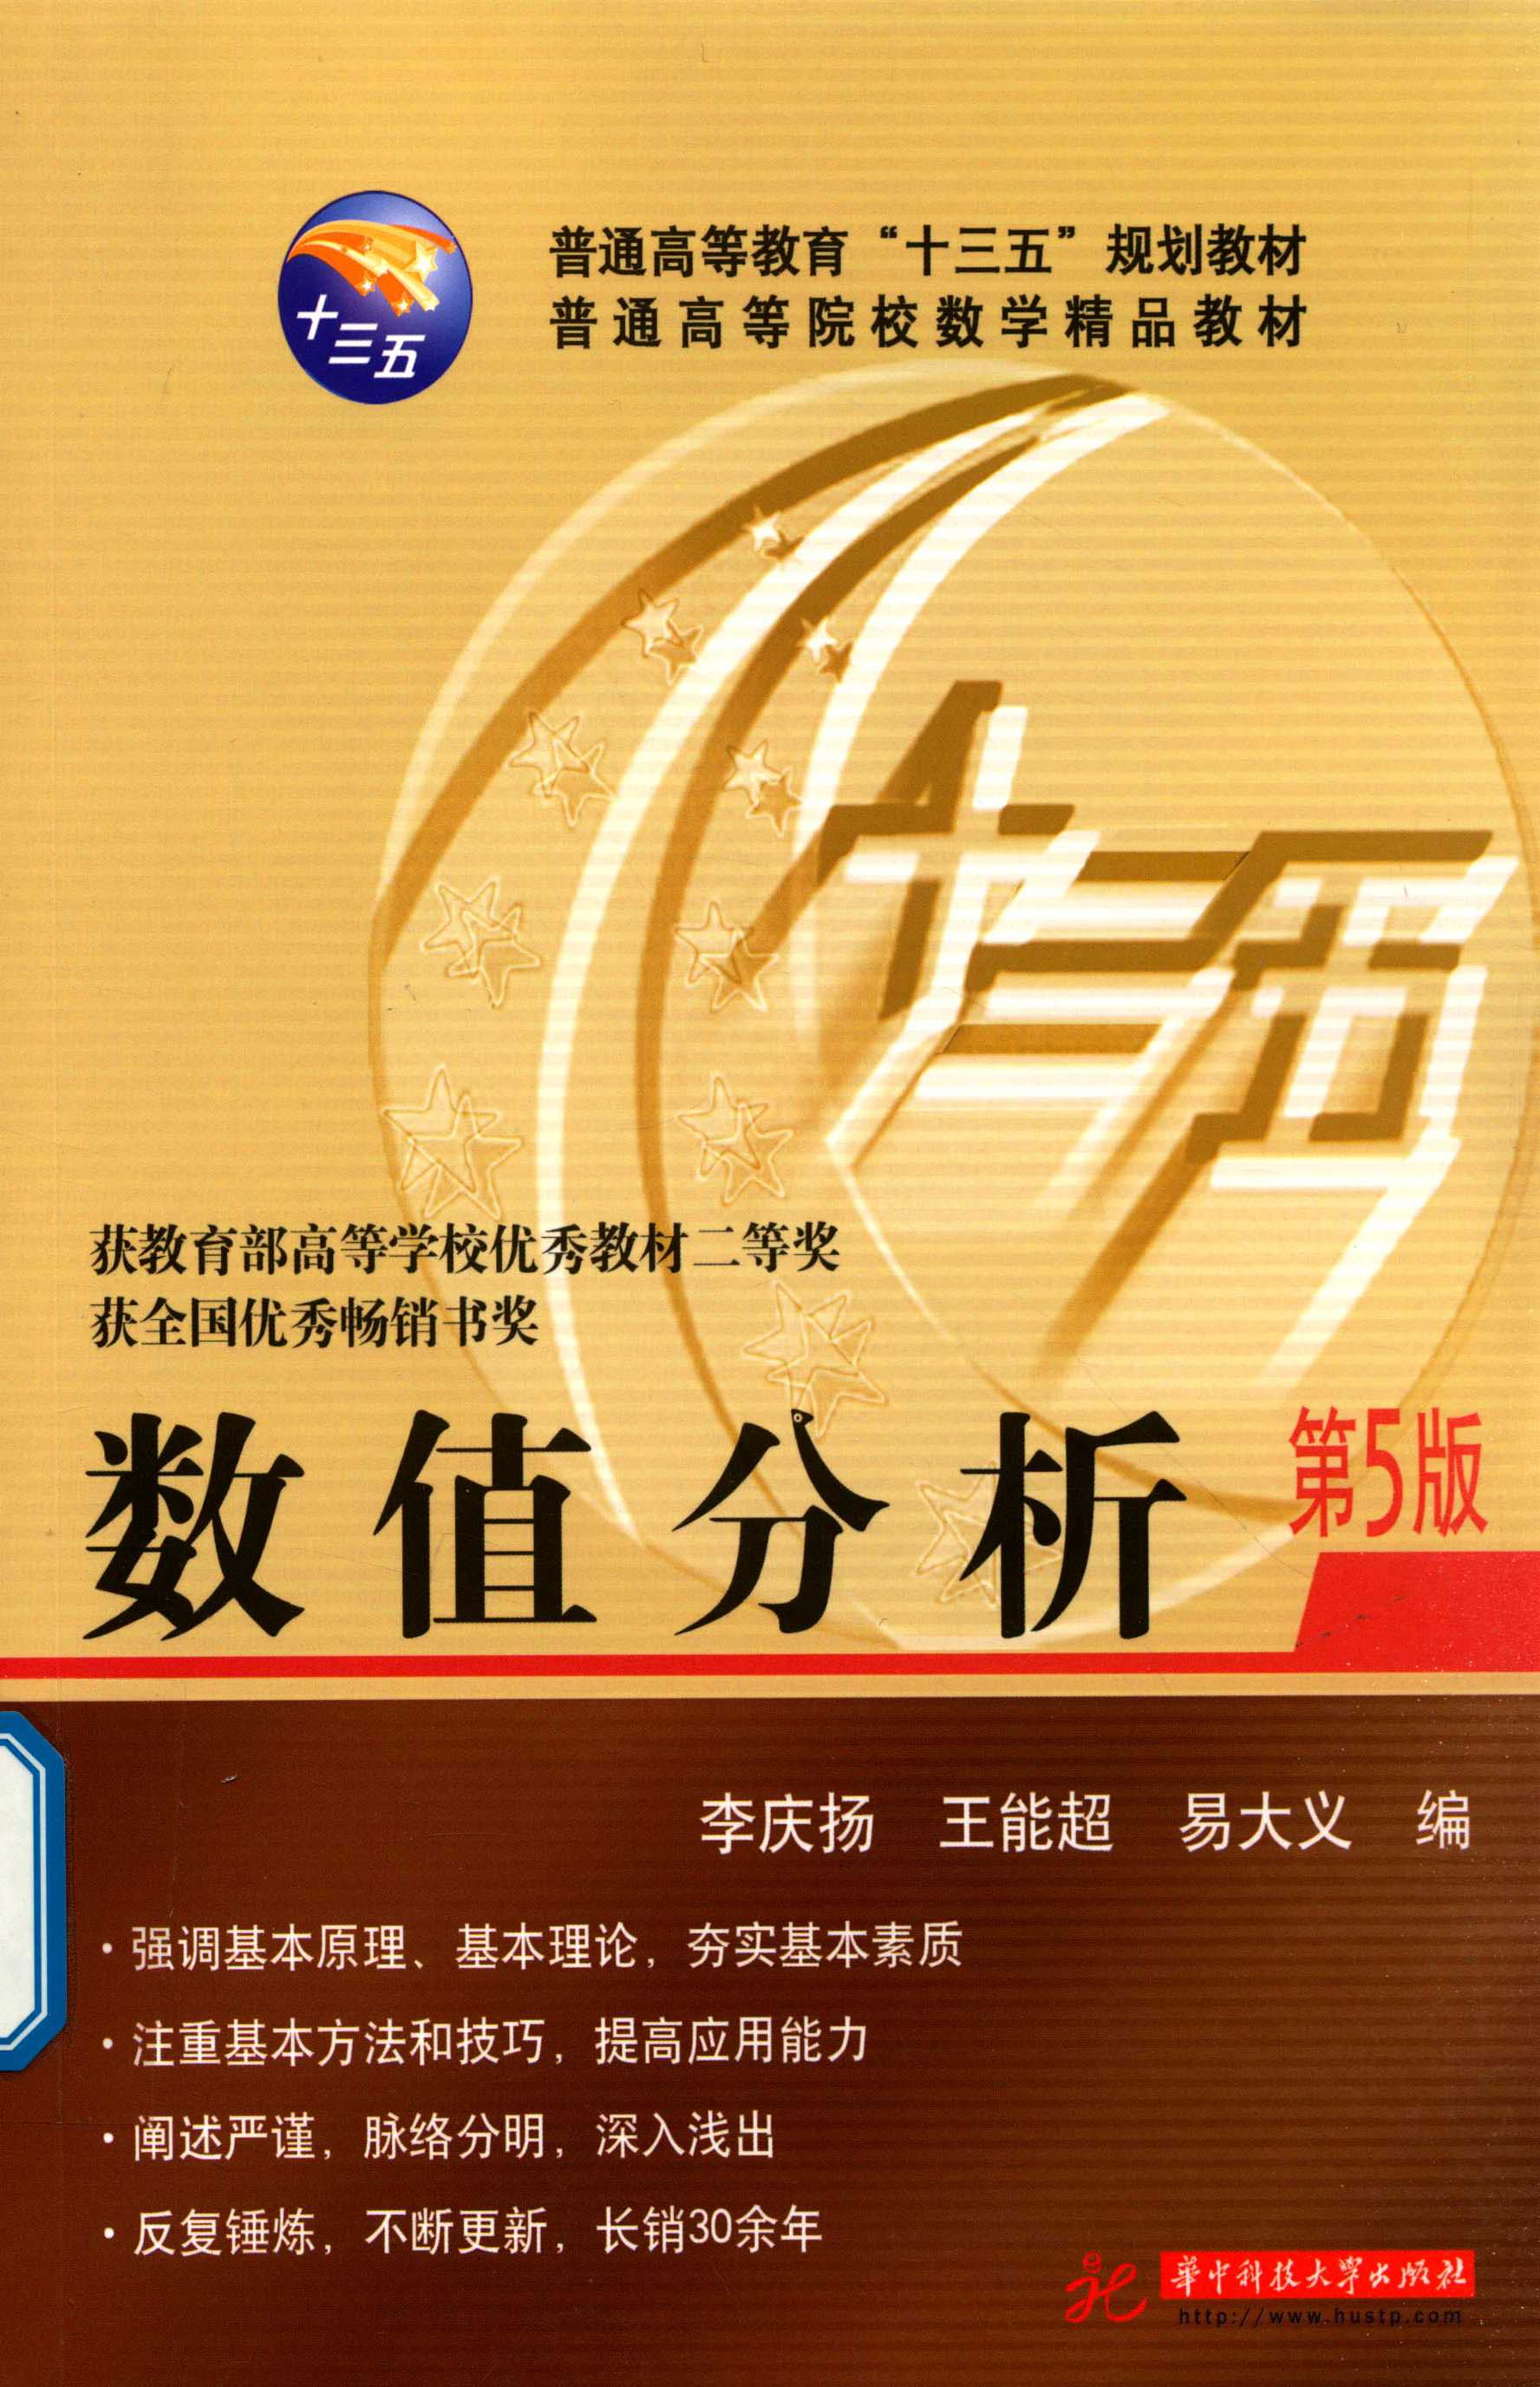
\includegraphics[width=0.85\linewidth,height=\textheight,keepaspectratio,alt={封面原图；含``十三五''徽标、背景装饰与出版社标识}]{verified/assets/front/cover-original.png}

\clearpage

原书 PDF 页 2；无印刷页码。

\href{source-images/pdf-002.jpeg}{查看原页}

普通高等教育``十三五''规划教材\\
普通高等院校数学精品教材

\section{数值分析（第 5 版）}\label{front-ux6570ux503cux5206ux6790ux7b2c-5-ux7248}

------数值算法分析与高效算法设计

李庆扬　王能超　易大义　编

华中科技大学出版社\\
中国·武汉

\clearpage

原书 PDF 页 3；无印刷页码。

\href{source-images/pdf-003.jpeg}{查看原页}

\section{内容提要}\label{front-ux5185ux5bb9ux63d0ux8981}

本书是为理工科院校各专业普遍开设的``数值分析''课程而编写的教材。其上篇内容包括插值与逼近、数值积分与数值微分、常微分方程与线性方程组的数值解法、矩阵的特征值与特征向量计算等。每章附有习题并在书末给出部分答案。

本书下篇（高效算法设计）以讲座形式介绍快速算法、并行算法与加速算法方面的几个典型案例，力图普及推广超级计算方面的基础知识。全书阐述严谨，脉络分明，深入浅出，便于教学。

本书可作为理工科院校应用数学、力学、物理、计算机等专业的教材，也可供从事科学计算的科技工作者参考。

\subsection{图书在版编目（CIP）数据}\label{front-ux56feux4e66ux5728ux7248ux7f16ux76eecipux6570ux636e}

数值分析／李庆扬，王能超，易大义编．---5 版．---武汉：华中科技大学出版社，2018.4\\
ISBN 978-7-5680-3946-8

Ⅰ．①数\ldots{}　Ⅱ．①李\ldots{}　②王\ldots{}　③易\ldots{}　Ⅲ．①数值分析-高等学校-教材　Ⅳ．①O241

中国版本图书馆 CIP 数据核字（2018）第 060527 号

\subsection{数值分析（第 5 版）}\label{front-ux6570ux503cux5206ux6790ux7b2c-5-ux7248-1}

Shuzhi Fenxi

李庆扬　王能超　易大义　编

{\def\LTcaptype{none} % do not increment counter
\begin{longtable}[]{@{}ll@{}}
\toprule\noalign{}
项目 & 内容 \\
\midrule\noalign{}
\endhead
\bottomrule\noalign{}
\endlastfoot
策划编辑 & 王汉江 \\
责任编辑 & 王汉江 \\
封面设计 & 原色设计 \\
责任校对 & 张会军 \\
责任监印 & 周治超 \\
出版发行 & 华中科技大学出版社（中国·武汉） \\
地址 & 武汉市东湖新技术开发区华工科技园 \\
电话 & (027)81321913 \\
邮编 & 430223 \\
录排 & 武汉市洪山区佳年华文印部 \\
印刷 & 武汉华工鑫宏印务有限公司 \\
开本 & \(710\,\mathrm{mm}\times1000\,\mathrm{mm}\)　\(1/16\) \\
印张 & 20 \\
字数 & 415 千字 \\
版次 & 2018 年 4 月第 5 版第 1 次印刷 \\
定价 & 39.80 元 \\
\end{longtable}
}


\includegraphics[width=0.25\linewidth,height=\textheight,keepaspectratio,alt={出版社标志原图：华中出版}]{verified/assets/front/publisher-mark-original.png}

华中出版

本书若有印装质量问题，请向出版社营销中心调换\\
全国免费服务热线：400-6679-118　竭诚为您服务\\
版权所有　侵权必究

\clearpage

原书 PDF 页 4；无印刷页码。

\href{source-images/pdf-004.jpeg}{查看原页}

\section{第 5 版前言}\label{front-ux7b2c-5-ux7248ux524dux8a00}

本书于 1981 年由华中科技大学出版社出版，至今已有 37 年。本书 1988 年获国家教委优秀教材二等奖，在国内为许多高校所选用。

今天，数值计算已进入超级计算的新时代，科技革命迅猛发展的新形势迫切要求普及推广高性能计算方面的新知识，鉴于这一认识本书推出第 5 版。

作为高效算法设计的关键技术，二分演化技术具有深邃的文化内涵，其设计思想新奇而玄妙，这方面内容可能尚未为人们所熟悉，笔者深信它处于算法设计学的前沿，因此选取快速算法设计、并行算法设计和加速算法设计方面的几个典型案例，汇集成讲座资料作为本书第 10～13 章，奉献给立志于从事高性能计算的读者参考。

本书中的第 10～13 章（讲座资料）由王能超撰写，错误与不当之处请读者不吝指正。

本书的再版，得到华中科技大学出版社的鼎力支持，在此表示衷心的感谢！

作者\\
2018 年 1 月

\clearpage

原书 PDF 页 5；无印刷页码。

\href{source-images/pdf-005.jpeg}{查看原页}

\section{第 2 版前言}\label{front-ux7b2c-2-ux7248ux524dux8a00}

1980 年 7 月在大连召开的工科院校``应用数学专业教学学术会议''，根据教育部直属工科院校``应用数学专业教学计划''制定了``数值分析''课大纲，并决定由清华大学、华中工学院、浙江大学合编试用教材。本书就是根据这次会议的决定编写的。全书共分 9 章，第 1～3 章由李庆扬编写，第 4～6 章由王能超编写，第 7～9 章由易大义编写。教材初稿于 1980 年 12 月投交华中工学院出版社。

1981 年元月在杭州召开的工科院校计算数学第一次教材审稿会，对本书初稿进行了审查，1982 年元月在上海交通大学召开的第二次计算数学教材审稿会，又对本书第 1 版提出了修改意见。会议考虑到理工科院校各专业普遍开设``数值分析''课的情况，重新修订了大纲（72 学时）。本书第 2 版就是根据新大纲的要求修改的，它保持了第 1 版的主要内容及特点，但选材更注意基本要求，减少了部分内容，增加了部分习题答案。本书可作为理工科院校应用数学、力学、物理、计算机软件等专业大学生及其他专业研究生``数值分析''（或``计算方法''）课的教材，也可供学习``计算方法''的科技工作者参考。

我们对参加两次审稿会的同志表示衷心感谢，他们以认真负责的态度对本书提出了许多宝贵意见，对提高教材质量起了很大作用。

编者\\
1982 年 7 月

\clearpage

原书 PDF 页 6；印刷页码 1。

\href{source-images/pdf-006.jpeg}{查看原页}

\section{目录}\label{front-ux76eeux5f55}

\begin{quote}
转录说明（agent 补充）：以下为印刷目录；末列是目录所列的正文书页码。本页底部的目录页码另记在 YAML 中。
\end{quote}

\subsection{上篇　数值算法分析}\label{front-ux4e0aux7bc7-ux6570ux503cux7b97ux6cd5ux5206ux6790}

{\def\LTcaptype{none} % do not increment counter
\begin{longtable}[]{@{}llr@{}}
\toprule\noalign{}
编号 & 标题 & 书页码 \\
\midrule\noalign{}
\endhead
\bottomrule\noalign{}
\endlastfoot
第 1 章 & \textbf{绪论} & 1 \\
1.1 & 数值分析研究的对象与特点 & 1 \\
1.2 & 误差来源与误差分析的重要性 & 2 \\
1.3 & 误差的基本概念 & 4 \\
1.3.1 & 误差与误差限 & 4 \\
1.3.2 & 相对误差与相对误差限 & 5 \\
1.3.3 & 有效数字 & 6 \\
1.3.4 & 数值运算的误差估计 & 7 \\
1.4 & 数值运算中误差分析的方法与原则 & 9 \\
1.4.1 & 要避免除数绝对值远远小于被除数绝对值的除法 & 9 \\
1.4.2 & 要避免两相近数相减 & 10 \\
1.4.3 & 要防止大数``吃掉''小数 & 11 \\
1.4.4 & 注意简化计算步骤，减少运算次数 & 11 \\
& 小结 & 12 \\
& 习题 & 12 \\
第 2 章 & \textbf{插值法} & 14 \\
2.1 & 引言 & 14 \\
2.2 & Lagrange 插值 & 15 \\
2.2.1 & 插值多项式的存在唯一性 & 15 \\
2.2.2 & 线性插值与抛物插值 & 16 \\
2.2.3 & Lagrange 插值多项式 & 18 \\
2.2.4 & 插值余项 & 19 \\
2.3 & 逐次线性插值法 & 21 \\
2.4 & 差商与 Newton 插值公式 & 23 \\
2.4.1 & 差商及其性质 & 23 \\
2.4.2 & Newton 插值公式 & 24 \\
2.5 & 差分与等距节点插值公式 & 26 \\
2.5.1 & 差分及其性质 & 26 \\
2.5.2 & 等距节点插值公式 & 28 \\
2.6 & Hermite 插值 & 29 \\
\end{longtable}
}

\clearpage

原书 PDF 页 7；印刷页码 2。

\href{source-images/pdf-007.jpeg}{查看原页}

\section{目录（续）}\label{front-ux76eeux5f55ux7eed}

\begin{quote}
转录说明（agent 补充）：以下为印刷目录；末列是目录所列的正文书页码。本页底部的目录页码另记在 YAML 中。
\end{quote}

{\def\LTcaptype{none} % do not increment counter
\begin{longtable}[]{@{}llr@{}}
\toprule\noalign{}
编号 & 标题 & 书页码 \\
\midrule\noalign{}
\endhead
\bottomrule\noalign{}
\endlastfoot
2.7 & 分段低次插值 & 32 \\
2.7.1 & 多项式插值的问题 & 32 \\
2.7.2 & 分段线性插值 & 33 \\
2.7.3 & 分段三次 Hermite 插值 & 34 \\
2.8 & 三次样条插值 & 36 \\
2.8.1 & 三次样条函数 & 36 \\
2.8.2 & 三转角方程 & 37 \\
2.8.3 & 三弯矩方程 & 39 \\
2.8.4 & 计算步骤与例题 & 40 \\
2.8.5 & 三次样条插值的收敛性 & 41 \\
& 小结 & 42 \\
& 习题 & 43 \\
第 3 章 & \textbf{函数逼近与计算} & 45 \\
3.1 & 引言与预备知识 & 45 \\
3.1.1 & 问题的提出 & 45 \\
3.1.2 & Weierstrass 定理 & 46 \\
3.1.3 & 连续函数空间 \(C[a,b]\) & 47 \\
3.2 & 最佳一致逼近多项式 & 47 \\
3.2.1 & 最佳一致逼近多项式的存在性 & 47 \\
3.2.2 & Chebyshev 定理 & 48 \\
3.2.3 & 最佳一次逼近多项式 & 50 \\
3.3 & 最佳平方逼近 & 52 \\
3.3.1 & 内积空间 & 52 \\
3.3.2 & 函数的最佳平方逼近 & 54 \\
3.4 & 正交多项式 & 57 \\
3.4.1 & 正交化手续 & 57 \\
3.4.2 & Legendre 多项式 & 57 \\
3.4.3 & Chebyshev 多项式 & 60 \\
3.4.4 & 其他常用的正交多项式 & 62 \\
3.5 & 函数按正交多项式展开 & 63 \\
3.6 & 曲线拟合的最小二乘法 & 65 \\
3.6.1 & 一般的最小二乘逼近 & 65 \\
3.6.2 & 用正交函数作最小二乘拟合 & 69 \\
3.6.3 & 多元最小二乘拟合 & 71 \\
3.7 & Fourier 逼近与快速 Fourier 变换 & 71 \\
3.7.1 & 最佳平方三角逼近与三角插值 & 71 \\
\end{longtable}
}

\clearpage

原书 PDF 页 8；印刷页码 3。

\href{source-images/pdf-008.jpeg}{查看原页}

\section{目录（续）}\label{front-ux76eeux5f55ux7eed-1}

\begin{quote}
转录说明（agent 补充）：以下为印刷目录；末列是目录所列的正文书页码。本页底部的目录页码另记在 YAML 中。
\end{quote}

{\def\LTcaptype{none} % do not increment counter
\begin{longtable}[]{@{}llr@{}}
\toprule\noalign{}
编号 & 标题 & 书页码 \\
\midrule\noalign{}
\endhead
\bottomrule\noalign{}
\endlastfoot
3.7.2 & 快速 Fourier 变换 & 74 \\
& 小结 & 77 \\
& 习题 & 77 \\
第 4 章 & \textbf{数值积分与数值微分} & 80 \\
4.1 & 引言 & 80 \\
4.1.1 & 数值求积的基本思想 & 80 \\
4.1.2 & 代数精度的概念 & 81 \\
4.1.3 & 插值型的求积公式 & 82 \\
4.2 & Newton-Cotes 公式 & 82 \\
4.2.1 & Cotes 系数 & 82 \\
4.2.2 & 偶阶求积公式的代数精度 & 84 \\
4.2.3 & 几种低阶求积公式的余项 & 85 \\
4.2.4 & 复化求积法及其收敛性 & 86 \\
4.3 & Romberg 算法 & 88 \\
4.3.1 & 梯形法的递推化 & 88 \\
4.3.2 & Romberg 公式 & 89 \\
4.3.3 & Richardson 外推加速法 & 91 \\
4.3.4 & 梯形法的余项展开式 & 92 \\
4.4 & Gauss 公式 & 93 \\
4.4.1 & Gauss 点 & 94 \\
4.4.2 & Gauss-Legendre 公式 & 95 \\
4.4.3 & Gauss 公式的余项 & 96 \\
4.4.4 & Gauss 公式的稳定性 & 96 \\
4.4.5 & 带权的 Gauss 公式 & 97 \\
4.5 & 数值微分 & 99 \\
4.5.1 & 中点方法 & 99 \\
4.5.2 & 插值型的求导公式 & 100 \\
4.5.3 & 实用的五点公式 & 102 \\
4.5.4 & 样条求导 & 103 \\
& 小结 & 104 \\
& 习题 & 104 \\
第 5 章 & \textbf{常微分方程数值解法} & 106 \\
5.1 & 引言 & 106 \\
5.2 & Euler 方法 & 106 \\
5.2.1 & Euler 格式 & 106 \\
5.2.2 & 后退的 Euler 格式 & 108 \\
\end{longtable}
}

\clearpage

原书 PDF 页 9；印刷页码 4。

\href{source-images/pdf-009.jpeg}{查看原页}

\section{目录（续）}\label{front-ux76eeux5f55ux7eed-2}

\begin{quote}
转录说明（agent 补充）：以下为印刷目录；末列是目录所列的正文书页码。本页底部的目录页码另记在 YAML 中。
\end{quote}

{\def\LTcaptype{none} % do not increment counter
\begin{longtable}[]{@{}llr@{}}
\toprule\noalign{}
编号 & 标题 & 书页码 \\
\midrule\noalign{}
\endhead
\bottomrule\noalign{}
\endlastfoot
5.2.3 & 梯形格式 & 109 \\
5.2.4 & 改进的 Euler 格式 & 110 \\
5.2.5 & Euler 两步格式 & 111 \\
5.3 & Runge-Kutta 方法 & 113 \\
5.3.1 & Taylor 级数法 & 113 \\
5.3.2 & Runge-Kutta 方法的基本思想 & 114 \\
5.3.3 & 二阶 Runge-Kutta 方法 & 115 \\
5.3.4 & 三阶 Runge-Kutta 方法 & 116 \\
5.3.5 & 四阶 Runge-Kutta 方法 & 118 \\
5.3.6 & 变步长的 Runge-Kutta 方法 & 119 \\
5.4 & 单步法的收敛性和稳定性 & 120 \\
5.4.1 & 单步法的收敛性 & 120 \\
5.4.2 & 单步法的稳定性 & 122 \\
5.5 & 线性多步法 & 124 \\
5.5.1 & 基于数值积分的构造方法 & 124 \\
5.5.2 & Adams 显式格式 & 125 \\
5.5.3 & Adams 隐式格式 & 126 \\
5.5.4 & Adams 预测-校正系统 & 127 \\
5.5.5 & 基于 Taylor 展开的构造方法 & 128 \\
5.5.6 & Milne 格式 & 130 \\
5.5.7 & Hamming 格式 & 131 \\
5.6 & 方程组与高阶方程的情形 & 132 \\
5.6.1 & 一阶方程组 & 132 \\
5.6.2 & 化高阶方程组为一阶方程组 & 133 \\
5.7 & 边值问题的数值解法 & 134 \\
5.7.1 & 试射法 & 135 \\
5.7.2 & 差分方程的建立 & 135 \\
5.7.3 & 差分问题的可解性 & 137 \\
5.7.4 & 差分方法的收敛性 & 138 \\
& 小结 & 140 \\
& 习题 & 140 \\
第 6 章 & \textbf{方程求根} & 142 \\
6.1 & 根的搜索 & 142 \\
6.1.1 & 逐步搜索法 & 142 \\
6.1.2 & 二分法 & 142 \\
6.2 & 迭代法 & 144 \\
\end{longtable}
}

\clearpage

原书 PDF 页 10；印刷页码 5。

\href{source-images/pdf-010.jpeg}{查看原页}

\section{目录（续）}\label{front-ux76eeux5f55ux7eed-3}

\begin{quote}
转录说明（agent 补充）：以下为印刷目录；末列是目录所列的正文书页码。本页底部的目录页码另记在 YAML 中。
\end{quote}

{\def\LTcaptype{none} % do not increment counter
\begin{longtable}[]{@{}llr@{}}
\toprule\noalign{}
编号 & 标题 & 书页码 \\
\midrule\noalign{}
\endhead
\bottomrule\noalign{}
\endlastfoot
6.2.1 & 迭代过程的收敛性 & 144 \\
6.2.2 & 迭代公式的加工 & 147 \\
6.3 & Newton 法 & 149 \\
6.3.1 & Newton 公式 & 149 \\
6.3.2 & Newton 法的几何解释 & 150 \\
6.3.3 & Newton 法的局部收敛性 & 151 \\
6.3.4 & Newton 法应用举例 & 152 \\
6.3.5 & Newton 下山法 & 153 \\
6.4 & 弦截法与抛物线法 & 154 \\
6.4.1 & 弦截法 & 155 \\
6.4.2 & 抛物线法 & 156 \\
6.5 & 代数方程求根 & 158 \\
6.5.1 & 多项式求值的秦九韶算法 & 158 \\
6.5.2 & 代数方程的 Newton 法 & 159 \\
6.5.3 & 劈因子法 & 160 \\
& 小结 & 162 \\
& 习题 & 162 \\
第 7 章 & \textbf{解线性方程组的直接方法} & 164 \\
7.1 & 引言 & 164 \\
7.2 & Gauss 消去法 & 164 \\
7.2.1 & 消元手续 & 165 \\
7.2.2 & 矩阵的三角分解 & 168 \\
7.2.3 & 计算量 & 170 \\
7.3 & Gauss 主元素消去法 & 171 \\
7.3.1 & 完全主元素消去法 & 172 \\
7.3.2 & 列主元素消去法 & 173 \\
7.3.3 & Gauss-Jordan 消去法 & 175 \\
7.4 & Gauss 消去法的变形 & 178 \\
7.4.1 & 直接三角分解法 & 178 \\
7.4.2 & 平方根法 & 181 \\
7.4.3 & 追赶法 & 184 \\
7.5 & 向量和矩阵的范数 & 186 \\
7.6 & 误差分析 & 192 \\
7.6.1 & 矩阵的条件数 & 192 \\
7.6.2 & 舍入误差 & 197 \\
& 小结 & 198 \\
\end{longtable}
}

\clearpage

原书 PDF 页 11；印刷页码 6。

\href{source-images/pdf-011.jpeg}{查看原页}

\section{目录（续）}\label{front-ux76eeux5f55ux7eed-4}

\begin{quote}
转录说明（agent 补充）：以下为印刷目录；末列是目录所列的正文书页码。本页底部的目录页码另记在 YAML 中。
\end{quote}

{\def\LTcaptype{none} % do not increment counter
\begin{longtable}[]{@{}llr@{}}
\toprule\noalign{}
编号 & 标题 & 书页码 \\
\midrule\noalign{}
\endhead
\bottomrule\noalign{}
\endlastfoot
& 习题 & 〔扫描残损；末位可辨为 8〕 \\
第 8 章 & \textbf{解线性方程组的迭代法} & 202 \\
8.1 & 引言 & 202 \\
8.2 & Jacobi 迭代法与 Gauss-Seidel 迭代法 & 204 \\
8.2.1 & Jacobi 迭代法 & 204 \\
8.2.2 & Gauss-Seidel 迭代法 & 205 \\
8.3 & 迭代法的收敛性 & 206 \\
8.4 & 解线性方程组的超松弛迭代法 & 213 \\
& 小结 & 217 \\
& 习题 & 217 \\
第 9 章 & \textbf{矩阵的特征值与特征向量计算} & 220 \\
9.1 & 引言 & 220 \\
9.2 & 幂法及反幂法 & 222 \\
9.2.1 & 幂法 & 222 \\
9.2.2 & 加速方法 & 225 \\
9.2.3 & 反幂法 & 227 \\
9.3 & Householder 方法 & 230 \\
9.3.1 & 引言 & 230 \\
9.3.2 & 用正交相似变换约化矩阵 & 232 \\
9.4 & QR 算法 & 237 \\
9.4.1 & 引言 & 237 \\
9.4.2 & QR 算法 & 239 \\
9.4.3 & 带原点位移的 QR 方法 & 242 \\
& 小结 & 246 \\
& 习题 & 246 \\
\end{longtable}
}

\subsection{下篇　高效算法设计}\label{front-ux4e0bux7bc7-ux9ad8ux6548ux7b97ux6cd5ux8bbeux8ba1}

{\def\LTcaptype{none} % do not increment counter
\begin{longtable}[]{@{}llr@{}}
\toprule\noalign{}
编号 & 标题 & 书页码 \\
\midrule\noalign{}
\endhead
\bottomrule\noalign{}
\endlastfoot
*第 10 章 & \textbf{快速算法设计:快速 Walsh 变换} & 248 \\
10.1 & 美的 Walsh 函数 & 248 \\
10.1.1 & 微积分的逼近法 & 248 \\
10.1.2 & Walsh 函数的复杂性 & 249 \\
10.1.3 & Walsh 分析的数学美 & 250 \\
10.2 & Walsh 函数代数化 & 251 \\
10.2.1 & 时基上的二分集 & 251 \\
10.2.2 & Walsh 函数的矩阵表示 & 252 \\
\end{longtable}
}

\begin{quote}
校注（agent 补充）：第 7 章``习题''的目录页码前部残损，末位可辨为 8；不能从本页确认其完整原印数字。正文起始处已回查为 PDF 第 212 页、书页 199，该正文定位不冒充目录原印页码。
\end{quote}

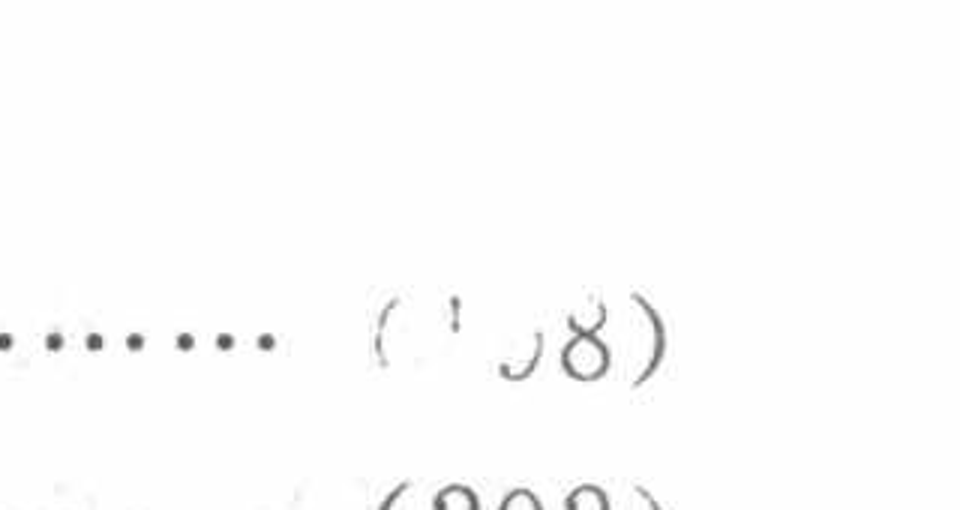
\includegraphics[width=0.85\linewidth,height=\textheight,keepaspectratio,alt={第7章习题目录页码原扫描局部，前部残损、末位可辨为8}]{verified/assets/front/toc-ch7-exercises-page-damage.png}

\href{source-images/pdf-212.jpeg}{正文``习题''起始页与书页 199}

\clearpage

原书 PDF 页 12；印刷页码 7。

\href{source-images/pdf-012.jpeg}{查看原页}

\section{目录（续）}\label{front-ux76eeux5f55ux7eed-5}

\begin{quote}
转录说明（agent 补充）：以下为印刷目录；末列是目录所列的正文书页码。本页底部的目录页码另记在 YAML 中。
\end{quote}

{\def\LTcaptype{none} % do not increment counter
\begin{longtable}[]{@{}llr@{}}
\toprule\noalign{}
编号 & 标题 & 书页码 \\
\midrule\noalign{}
\endhead
\bottomrule\noalign{}
\endlastfoot
10.3 & Walsh 阵的二分演化 & 252 \\
10.3.1 & 矩阵的对称性复制 & 253 \\
10.3.2 & Walsh 阵的演化生成 & 253 \\
10.3.3 & Walsh 阵的演化机制 & 254 \\
10.3.4 & Hadamard 阵的演化生成 & 255 \\
10.4 & 快速变换 FWT & 257 \\
10.4.1 & FWT 的设计思想 & 257 \\
10.4.2 & FWT 的演化机制 & 258 \\
10.4.3 & FWT 的计算流程 & 259 \\
10.4.4 & FWT 的算法实现 & 261 \\
& 小结 & 262 \\
*第 11 章 & \textbf{并行算法设计:递推计算并行化} & 263 \\
11.1 & 什么是并行计算 & 263 \\
11.1.1 & 一则寓言故事 & 263 \\
11.1.2 & 同步并行算法的设计策略 & 264 \\
11.2 & 叠加计算 & 265 \\
11.2.1 & 倍增技术 & 265 \\
11.2.2 & 二分手续 & 267 \\
11.2.3 & 数列求和的二分法 & 268 \\
11.2.4 & 多项式求值的二分法 & 269 \\
11.2.5 & 二分算法的效能分析 & 270 \\
11.2.6 & 二分算法的基本特征 & 271 \\
11.3 & 一阶线性递推 & 272 \\
11.3.1 & 相关链的二分手续 & 272 \\
11.3.2 & 算式的建立 & 273 \\
11.3.3 & 二分算法的效能分析 & 275 \\
11.4 & 三对角方程组 & 275 \\
11.4.1 & 相关链的二分手续 & 276 \\
11.4.2 & 算式的建立 & 277 \\
& 小结 & 279 \\
*第 12 章 & \textbf{加速算法设计:重差加速技术} & 281 \\
12.1 & 千古疑案 & 281 \\
12.1.1 & 阿基米德的``穷竭法'' & 281 \\
12.1.2 & 祖冲之``缀术''之谜 & 281 \\
12.2 & 神来之笔 & 282 \\
\end{longtable}
}

\clearpage

原书 PDF 页 13；印刷页码 8。

\href{source-images/pdf-013.jpeg}{查看原页}

\section{目录（续）}\label{front-ux76eeux5f55ux7eed-6}

\begin{quote}
转录说明（agent 补充）：以下为印刷目录；末列是目录所列的正文书页码。本页底部的目录页码另记在 YAML 中。
\end{quote}

{\def\LTcaptype{none} % do not increment counter
\begin{longtable}[]{@{}llr@{}}
\toprule\noalign{}
编号 & 标题 & 书页码 \\
\midrule\noalign{}
\endhead
\bottomrule\noalign{}
\endlastfoot
12.2.1 & 数学史上一篇千古奇文 & 282 \\
12.2.2 & ``一飞冲天''的``刘徽神算'' & 283 \\
12.3 & 奇光异彩 & 284 \\
12.3.1 & 刘徽的新视野 & 285 \\
12.3.2 & 偏差比中传出好``消息'' & 286 \\
12.3.3 & 只要做一次``俯冲'' & 286 \\
12.3.4 & 差之毫厘,失之千里 & 287 \\
12.3.5 & ``缀术''再剖析 & 288 \\
12.3.6 & 平庸的新纪录 & 289 \\
12.4 & 万能引擎 & 291 \\
12.4.1 & 逼近加速的重差公设 & 292 \\
12.4.2 & 重差加速法则 & 292 \\
12.4.3 & 重差加速的逻辑推理 & 293 \\
第 13 章 & \textbf{总览} & 294 \\
13.1 & 算法重在设计 & 294 \\
13.1.1 & 算法设计关系到科学计算的成败 & 294 \\
13.1.2 & 算法设计追求简单与统一 & 295 \\
13.2 & 直接法的缩减技术 & 295 \\
13.2.1 & 数列求和的累加算法 & 295 \\
13.2.2 & 缩减技术的设计机理 & 296 \\
13.2.3 & 多项式求值的秦九韶算法 & 297 \\
13.3 & 迭代法的校正技术 & 298 \\
13.3.1 & 开方算法 & 298 \\
13.3.2 & 校正技术的设计机理 & 299 \\
13.4 & 迭代优化的超松弛技术 & 300 \\
13.4.1 & 超松弛技术的设计机理 & 300 \\
13.4.2 & 刘徽的``割圆术'' & 300 \\
13.5 & 递推加速的二分技术 & 301 \\
13.5.1 & ``结绳记数''的快速算法 & 301 \\
13.5.2 & 二分技术的设计机理 & 302 \\
& 小结 & 303 \\
& 部分习题答案 & 305 \\
& 参考文献 & 308 \\
\end{longtable}
}

